%----------------------------------------------------------------------------------------
%	PACKAGES AND OTHER DOCUMENT CONFIGURATIONS
%----------------------------------------------------------------------------------------

\documentclass{scrartcl}

\reversemarginpar

\newcommand{\MarginText}[1]{\marginpar{\raggedleft\itshape\small#1}}

\usepackage[nochapters]{classicthesis}
\usepackage[LabelsAligned,NoDate]{currvita}

\usepackage{graphicx}
\usepackage[export]{adjustbox}
\pagenumbering{gobble}

\definecolor{cvblue}{RGB}{13,27,76}

\renewcommand{\cvheadingfont}{\LARGE\color{cvblue}}

\usepackage{hyperref}
\hypersetup{colorlinks, breaklinks, urlcolor=cvblue, linkcolor=cvblue}

\newlength{\datebox}\settowidth{\datebox}{2010/01--2011/01}

\newcommand{\NewEntry}[3]{\noindent\hangindent=2em\hangafter=0 \MarginText{#1}#2 #3 \par\vspace{0.5em}}
\newcommand{\InfoEntry}[3]{\noindent\hangindent=2em\hangafter=0 \parbox{\datebox}{\small \textit{#1}}\hspace{1.5em} #2 #3 \par}

\newcommand{\Description}[1]{\hangindent=2em\hangafter=0\noindent\raggedright\footnotesize{#1}\par\normalsize\vspace{1em}}

\newcommand{\cvsection}[1]{\noindent\spacedlowsmallcaps{#1}\par\vspace{1em}}
\setlength{\marginparsep}{-1em}


%----------------------------------------------------------------------------------------

\usepackage{eso-pic}
\newcommand\BackgroundPic{%
  \put(\LenToUnit{0pt},\LenToUnit{\dimexpr\paperheight-4pt\relax}){%
    \color{cvblue}\rule{\paperwidth}{4pt}%
  }%
}

\newcommand\Mugshot{\put(-112,290){\parbox[b][\paperheight]{\paperwidth}{%
\vfill\centering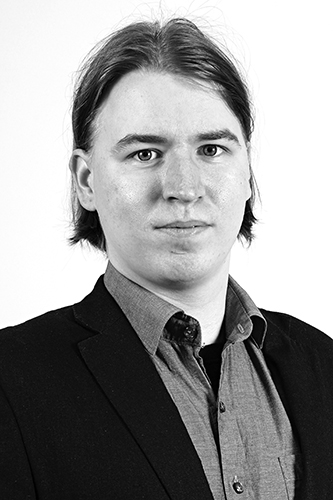
\includegraphics[width=\paperwidth,height=100pt,keepaspectratio]{mugshot.jpg}%
\vfill
}}}

\usepackage{fontawesome5}
\usepackage{needspace}

\begin{document}
\thispagestyle{empty}

%----------------------------------------------------------------------------------------
%	NAME AND CONTACT INFORMATION SECTION
%----------------------------------------------------------------------------------------
\begin{cv}{\textbf{\spacedallcaps{Santeri Lehtonen}}}\vspace{1.5em}
\AddToShipoutPicture*{\BackgroundPic}
\AddToShipoutPicture*{\Mugshot}
\cvsection{Personal Information}

\InfoEntry{}{\textit{Born in Finland,}}{8th of November, 1993} 

\InfoEntry{}{\faEnvelope \hspace{0.5em} \href{mailto:santeri@lehtone.nl}{santeri@lehtone.nl}}{} 

\InfoEntry{}{\faPhone \hspace{0.5em} +358 50 464 5751}{}

\InfoEntry{}{\faInstagram \hspace{0.5em} \href{https://www.instagram.com/_sntr_/}{\_sntr\_}}{}
\InfoEntry{}{\faLinkedin \hspace{0.5em} \href{https://www.linkedin.com/in/santerilehtonen/}{santerilehtonen}}{}
\InfoEntry{}{\faGithub \hspace{0.5em} \href{https://github.com/sntr8}{sntr8}}{}

\vspace{3em}

\cvsection{Profile}
\Description{For the last several years DevOps has been the main focus: building and running infrastructure, automating what can be automated, and keeping production reliable. Most of my consulting has been with finance and government clients, where reliability and security genuinely matter. Day to day that means a lot of Ansible, Linux, and Docker, with AWS for the public cloud pieces; at Eficode I built a private cloud platform for a finance client and continue to manage its lifecycle, middleware, and security.

\par\vspace{0.5em}
Earlier in my career I spent several years in identity and access management, working on user provisioning, single sign-on with SAML and OAuth, GDPR compliance, and large SQL databases. That background still informs how I think about access and data.}

%----------------------------------------------------------------------------------------
%	WORK EXPERIENCE
%----------------------------------------------------------------------------------------

\cvsection{Work Experience}

\needspace{5em}
\NewEntry{2019/08--Present}{Senior DevOps Consultant, \textsc{Eficode Oy}}{}
\Description{\MarginText{}I am currently working as a CI/CD and DevOps consultant. As the Lead Developer for a private cloud solution in the finance sector, I built a platform where servers can be ordered and provisioned automatically according to user needs. I manage their cloud platform lifecycle, middleware installations, security, and keep Ansible playbooks up-to-date. I have also led a project digitalizing access right forms for a government agency and improved DevOps methodologies for the IAM team.}

%------------------------------------------------

\needspace{5em}
\NewEntry{2007--Present}{Entrepreneur (IT Services \& AV Production), \textsc{SRSTI Consulting / sntrLXdesigns}}{}
\Description{\MarginText{}I run my own business providing comprehensive IT solutions, custom software development, and professional AV services. On the IT side, I manage Linux servers and web hosting for small businesses, handle DNS routing via AWS Route 53, administer Google Workspace (G-Suite) environments, and build bespoke web applications for clients, including a live production work order management system for a concrete pumping company. 

\par\vspace{0.5em}
In addition to IT services, I work extensively as a freelance lighting technician, operator, and designer. Currently, I mainly work at Messukeskus and tour continuously with Antti Ketonen, but also find myself at different venues in Southern Finland doing corporate events, concerts, musicals, and festivals. I have worked at multiple Tuska festivals, Nordic Business Forums, and Slush events, and have served as a lighting designer and operator for Assembly Computer Festival events since 2010. I have extensive knowledge of the MA Lighting MA3 system and train new operators online.}

%------------------------------------------------

\needspace{5em}
\NewEntry{2017/04--2019/08}{Solution Consultant \& Advisor, \textsc{Efecte Finland Oy}}{}
\Description{\MarginText{}I worked across Professional Services, Service Advisory, and Customer Success. My tasks varied from helping customers deploy new IdM solutions to providing 2nd level support, performing root-cause analysis of critical production bugs and architectural bottlenecks in production environments. \\I also worked closely with the Cloud Operations team running and improving our Docker-based cloud solution, and was part of the team creating internal DevOps procedures, including Jira and Bitbucket integrations.}

%------------------------------------------------

\needspace{5em}
\NewEntry{2017/01--2017/4}{Consultant, \textsc{WeAre Solutions Oy}}{}
\Description{\MarginText{}I worked as an identity and access management consultant. During my brief stay, I built a password reset service for external users of a financial company. I also created an Ansible playbook for deploying access management software on an existing server for mobile online banking authentication services.}

%------------------------------------------------

\needspace{5em}
\NewEntry{2016/01--2017/01}{Associate, \textsc{KPMG Oy Ab}}{}
\Description{\MarginText{}I worked as an identity management consultant. My work consisted of planning, developing, and implementing features for customers' existing and new IdM solutions.\\I was a part of the team developing the internal development workflow for the KPMG FI IAM division. The workflow included Git version control with advanced branch handling, code review processes, and automated configuration deployment to servers using the Ansible deployment tool. I also worked on automated installations of IdM environments, creating Ansible playbooks to install IdM software, databases, and application servers.}

%------------------------------------------------

\needspace{5em}
\NewEntry{2015/04--2015/12}{Junior Consultant, \textsc{Trusteq Oy}}{}
\Description{\MarginText{}I worked as a junior identity management consultant. My work consisted of planning, developing, and implementing features for customers' existing and new IdM solutions. I was transferred to work for KPMG after Trusteq was incorporated into KPMG.}

%------------------------------------------------

\needspace{3em}
\cvsection{Early Work History}

\Description{\MarginText{2014/05--2015/4}Chauffeur, \textsc{Taksikuljetus Oy}}
\Description{\MarginText{2013/09--2014/4}Taxi driver, \textsc{Tracent Oy}}
\Description{\MarginText{2012/11--2013/8}Construction assistant, \textsc{Suomen Rakennuslogistiikka Oy}}

%------------------------------------------------

\vspace{1em}

%----------------------------------------------------------------------------------------
%	PROJECTS
%----------------------------------------------------------------------------------------

\cvsection{Projects}

\needspace{10em}
\NewEntry{2020/12--2026/06}{Lead Developer --- Private Cloud Automation, \textsc{Confidential (Finance Sector)}}{}
\Description{\MarginText{}Acted as Lead Developer for engineering and automation of the client's private cloud infrastructure at Eficode. Orchestrated deployments utilizing Ansible and Ansible Automation Platform. Built robust CI/CD pipelines with Jenkins and ensured high-quality Infrastructure as Code by implementing automated unit testing for Ansible playbooks with Robot Framework. Managed strict monthly security releases to maintain platform integrity and financial industry compliance standards.\par\vspace{0.5em}\textit{Technologies: Ansible, Ansible Automation Platform, Linux, Red Hat Developer Hub, Robot Framework, Jenkins, Bash scripting}}

\needspace{8em}
\NewEntry{2020/11--2021/02}{Senior Consultant --- ITSM Transformation \& Asset Management, \textsc{Confidential (Chemical Industry)}}{}
\Description{\MarginText{}Worked on a comprehensive ITSM modernization project. Replaced outdated ticketing infrastructure with a unified Jira environment. Designed a JSM self-service portal for end-customers and implemented a centralized asset tracking system utilizing Jira Assets, integrating the company's entire mobile device inventory for improved visibility and lifecycle management.\par\vspace{0.5em}\textit{Technologies: Automation for Jira, Jira Software Cloud, Jira Service Management Cloud, Jira Assets}}

\needspace{8em}
\NewEntry{2019/08--2020/12}{DevOps Consultant --- Transformation \& Process Digitalization, \textsc{Confidential (Government Agency)}}{}
\Description{\MarginText{}Directed a dual-focus modernization initiative for a government agency, driving both cultural shifts and technical process improvements. Designed and delivered comprehensive DevOps transformation training for the customer's delivery team. Managed the digitalization of a legacy paper-based system access request process, deploying an automated, secure, and fully digital workflow ensuring strict compliance and auditability for government standards.\par\vspace{0.5em}\textit{Technologies: IAM, DevOps Transformation, Ansible}}

\needspace{10em}
\NewEntry{2026--}{Digital Work Order System, \textsc{Suomen Erikoispumppaus Oy} (via SRSTI Consulting)}{}
\Description{\MarginText{}Designed and built a tablet-friendly web application to replace a paper-based work order process for a concrete pumping company. Field drivers fill in work orders on site, with customer and equipment data auto-filling from a database. The system includes Google Workspace SSO with just-in-time role provisioning, autosave, and server-side PDF export. Deployed to a self-hosted Hetzner VPS behind an Apache reverse proxy, with a fully automated CI/CD pipeline via GitHub Actions building and deploying a Docker image on every push to main. Repository is private.\par\vspace{0.5em}\textit{Technologies: React, Vite, Tailwind CSS, Node.js, Express, MySQL, Knex.js, Docker, GitHub Actions, Google OAuth2, Apache, Puppeteer}}

\needspace{10em}
\NewEntry{2021--}{Docker-based RTMP restreamer}{}
\Description{\MarginText{}Developed a Docker-based RTMP restreaming solution to solve the security risk of multiple creators sharing a single static stream key. The system acts as a secure abstraction layer, hiding the master key from users and programmatically generating unique, time-restricted endpoints for each session. By automating the provisioning and de-provisioning of these transient stream keys, the solution prevents unauthorized access and ensures that content creators can only stream during their pre-specified time slots. The architecture utilizes a containerized stack including HAproxy, MySQL, and NGINX, fully managed via custom Python and Bash automation tools.\par\vspace{0.5em}\faGithub \hspace{0.5em} \href{https://github.com/sntr8/rtmp-proxy-server}{rtmp-proxy-server on GitHub}}

\needspace{8em}
\NewEntry{2023--2026}{Discord AM Bot}{}
\Description{\MarginText{}Engineered a Python-based Discord bot utilizing the Discord.py library to automate Identity and Access Management (IAM) for a large-scale gaming community. The bot features real-time synchronization with a tournament management system via HTTP APIs, automatically provisioning and de-provisioning server roles based on active player rosters. To ensure high availability and continuous delivery, the bot is deployed as a containerized service that is automatically rebuilt and redeployed to incorporate live updates.\par\vspace{0.5em}\faGithub \hspace{0.5em} \href{https://github.com/sntr8/discord-bots}{discord-bots on GitHub}}

\Description{\MarginText{}\textit{See LinkedIn profile for more project references.}}

\vspace{1em} % Extra space between major sections

%----------------------------------------------------------------------------------------
%	SKILLS
%----------------------------------------------------------------------------------------

\cvsection{Skills}

\Description{\MarginText{AI \& Data Engineering}AI-Assisted Development\ \ $\cdotp$\ \ AWS Bedrock\ \ $\cdotp$\ \ Claude (Anthropic)\ \ $\cdotp$\ \ GitHub Copilot\ \ $\cdotp$\ \ Google AI\ \ $\cdotp$\ \ LLM Integration\ \ $\cdotp$\ \ Prompt Engineering}

\Description{\MarginText{Atlassian \& ITSM}Atlassian Bitbucket\ \ $\cdotp$\ \ Atlassian Jira (Software, Service Management, Assets)\ \ $\cdotp$\ \ Confluence\ \ $\cdotp$\ \ Draw.io\ \ $\cdotp$\ \ Gliffy Diagrams\ \ $\cdotp$\ \ ITIL\ \ $\cdotp$\ \ ITSM\ \ $\cdotp$\ \ ServiceNow}

\Description{\MarginText{AWS}CloudWatch, EC2, ECS, EventBridge, IAM, Lambda, RDS, Route 53, S3, SES}

\Description{\MarginText{CI/CD \& Automation}\textbf{Ansible}\ \ $\cdotp$\ \ Ansible Automation Platform\ \ $\cdotp$\ \ GitHub Actions\ \ $\cdotp$\ \ GitLab CI\ \ $\cdotp$\ \ Jenkins\ \ $\cdotp$\ \ JMeter\ \ $\cdotp$\ \ Maven\ \ $\cdotp$\ \ Robot Framework\ \ $\cdotp$\ \ SonarQube}

\Description{\MarginText{Cloud \& Containers}\textbf{Docker}\ \ $\cdotp$\ \ Docker Compose\ \ $\cdotp$\ \ Azure\ \ $\cdotp$\ \ Azure DevOps\ \ $\cdotp$\ \ Elastic Stack (ELK)\ \ $\cdotp$\ \ Google Cloud Platform\ \ $\cdotp$\ \ Hashicorp Vault\ \ $\cdotp$\ \ Kubernetes\ \ $\cdotp$\ \ Rancher\ \ $\cdotp$\ \ Terraform}

\Description{\MarginText{Databases}\textbf{MySQL}\ \ $\cdotp$\ \ IBM DB2\ \ $\cdotp$\ \ MongoDB\ \ $\cdotp$\ \ Oracle SQL\ \ $\cdotp$\ \ PostgreSQL\ \ $\cdotp$\ \ SQLite}

\Description{\MarginText{Dev \& Scripting}\textbf{Python}\ \ $\cdotp$\ \ Bash / Shell scripting\ \ $\cdotp$\ \ BeanShell\ \ $\cdotp$\ \ CSS\ \ $\cdotp$\ \ Discord.py\ \ $\cdotp$\ \ Git\ \ $\cdotp$\ \ Groovy\ \ $\cdotp$\ \ HTML\ \ $\cdotp$\ \ HTTP API / REST\ \ $\cdotp$\ \ Java (EE/SE)\ \ $\cdotp$\ \ JavaScript\ \ $\cdotp$\ \ Jinja2\ \ $\cdotp$\ \ jQuery\ \ $\cdotp$\ \ JSON\ \ $\cdotp$\ \ \LaTeX\ \ $\cdotp$\ \ PHP\ \ $\cdotp$\ \ TypeScript\ \ $\cdotp$\ \ XML\ \ $\cdotp$\ \ YAML}

\Description{\MarginText{Identity \& Security}Efecte Identity Management\ \ $\cdotp$\ \ IAM\ \ $\cdotp$\ \ LDAP\ \ $\cdotp$\ \ SailPoint IdentityIQ\ \ $\cdotp$\ \ SAML SSO}

\Description{\MarginText{Infra \& OS}\textbf{Linux (Debian, RedHat)}\ \ $\cdotp$\ \ Certificate Lifecycle Management\ \ $\cdotp$\ \ Cloudflare\ \ $\cdotp$\ \ Grafana\ \ $\cdotp$\ \ Kibana\ \ $\cdotp$\ \ macOS\ \ $\cdotp$\ \ SELinux\ \ $\cdotp$\ \ Vagrant\ \ $\cdotp$\ \ VMware\ \ $\cdotp$\ \ Zabbix}

\Description{\MarginText{Methodologies \& Other}\textbf{MA Lighting MA3}\ \ $\cdotp$\ \ Adobe Photoshop\ \ $\cdotp$\ \ Agile\ \ $\cdotp$\ \ DevOps\ \ $\cdotp$\ \ Drools\ \ $\cdotp$\ \ Illustrator\ \ $\cdotp$\ \ iWork\ \ $\cdotp$\ \ Kanban\ \ $\cdotp$\ \ Microsoft Office\ \ $\cdotp$\ \ Red Hat Developer Hub\ \ $\cdotp$\ \ Scrum\ \ $\cdotp$\ \ Scrum Master\ \ $\cdotp$\ \ Trello\ \ $\cdotp$\ \ WordPress}

\Description{\MarginText{Middleware}Apache\ \ $\cdotp$\ \ HAProxy\ \ $\cdotp$\ \ JBoss AS\ \ $\cdotp$\ \ NGINX\ \ $\cdotp$\ \ Tomcat\ \ $\cdotp$\ \ WebLogic}

\Description{\MarginText{Quality}Unit Testing\ \ $\cdotp$\ \ System Testing\ \ $\cdotp$\ \ Acceptance Testing\ \ $\cdotp$\ \ Quality Assurance}

\Description{\MarginText{Compliance \& Regulations}GDPR\ \ $\cdotp$\ \ DORA (Digital Operational Resilience Act)}

\Description{\MarginText{Professional Skills}Corporate Governance\ \ $\cdotp$\ \ Information Architecture\ \ $\cdotp$\ \ Information Management\ \ $\cdotp$\ \ Integration\ \ $\cdotp$\ \ Presales Support\ \ $\cdotp$\ \ Secure Development\ \ $\cdotp$\ \ Security Clearance (Finland)}

\vspace{1em} % Extra space between major sections

%----------------------------------------------------------------------------------------
%	EDUCATION
%----------------------------------------------------------------------------------------

\needspace{5em}
\cvsection{Education and certificates}

\NewEntry{2019/10}{AWS Certified Cloud Practitioner, Amazon Web Services}{}
\Description{Credentials ID: Q5433VS13FB41FWN}
\NewEntry{2014}{GrandMA2 User Training, basic level, MA Lighting International GmbH}{}
\NewEntry{2009--2012}{Matriculation Examination, \textsc{L{\"a}nsi-Helsingin Lukio, Helsinki}}{}

%------------------------------------------------

\vspace{1em}

%------------------------------------------------

\cvsection{Other}

\vspace{1em}

\newlength{\langbox}
\settowidth{\langbox}{English}

\Description{\MarginText{Languages}\parbox{\langbox}{Finnish}\ \ $\cdotp$\ \ \ Native Proficiency}
\vspace{-0.5em} 
\Description{\parbox{\langbox}{English}\ \ $\cdotp$\ \ \ Full Working Proficiency}
\vspace{-0.5em} 
\Description{\parbox{\langbox}{Others}\ \ $\cdotp$\ \ \ Swedish (Limited Working)\ \ $\cdotp$\ \ \ Spanish, Italian, Russian (Basics)}

\vspace{1em}

\Description{\MarginText{Industry Experience}Financial Services\ \ $\cdotp$\ \ Government \& Public Sector\ \ $\cdotp$\ \ Manufacturing \& Logistics\ \ $\cdotp$\ \ Retail \& E-commerce\ \ $\cdotp$\ \ Technology \& IT Services}

\Description{\MarginText{Professional Interests}Generative AI Infrastructure\ \ $\cdotp$\ \ LLMOps\ \ $\cdotp$\ \ Public Cloud\ \ $\cdotp$\ \ Vector Database Architectures}

\Description{\MarginText{Hobbies}Computer gaming\ \ $\cdotp$\ \ Show lighting\ \ $\cdotp$\ \ Motorsport (Track day and go-kart)\ \ $\cdotp$\ \ Photography}

\Description{\MarginText{Driving License}B/C}

\needspace{8em}
\cvsection{Awards}
\NewEntry{2013/08}{The Best Organizer Award,}{\textsc{Assembly Summer 2013}}
\Description{I was awarded the Best Organizer award for LiveCrew at the Assembly Summer 2013 demoscene party. During the event, I was responsible for main stage lighting and helped out with AssemblyTV and seminars as well.}
\NewEntry{2013/02}{Honorary Award,}{\textsc{Assembly Winter 2013}}
\Description{I received an Honorary Award for my performance during the Assembly Winter 2013 computer gaming event, where I was responsible for main stage and hall lighting.}

\vfill
\centerline{\footnotesize Typeset in \LaTeX\ $\cdotp$\ \today}
\end{cv}

\end{document}